\documentclass[10pt,a4paper]{article}
\usepackage[utf8]{inputenc}
\usepackage[german]{babel}
\usepackage{amsmath}
\usepackage{amsfonts}
\usepackage{amssymb}
\usepackage{graphicx} %Um Bilder anzeigen zu können
\usepackage[top=1in, bottom=1.5in, left=1in, right=1in]{geometry}

\title{\Huge Pflichtenheft\\[1cm] {\bfseries Praxis der Softwareentwicklung}\\Gruppe 1\\[2cm] Entwicklung einer Software zur Berechnung der Mandatsverteilung im Deutschen Bundestag\\[1cm] }
\author{Philipp Löwer, Anton Mehlmann, Manuel Olk, Enes Ördek, \\Simon Schürg, Nick Vlasoff}
\date{}

\begin{document}
\maketitle

\begin{figure}[h]

\centering
		
		
\includegraphics[scale=0.6]{KIT-Logo.png}\\
		\Huge WS 2013 / 14
\end{figure}

		
\newpage
\tableofcontents
\newpage

\section{Produktübersicht}
Bei dem Produkt handelt es sich um ein Programm, das die Sitzverteilung im Deutschen Bundestag gemäß der gesetzlichen Bestimmungen exakt berechnet und deren Zustandekommen verständlich darlegt. Erreicht wird dies durch eine minimalistische und intuitive Benutzeroberfläche.

\subsection{Lizenz}
Der Quellcode des Programms wird der Öffentlichkeit frei zur Verfügung gestellt. Es wird die GPL V3 Lizenz verwendet, damit das Projekt nach einer Modifizierung weiterhin öffentlich bleibt.

\section{Zielbestimmung}
\subsection{Musskriterien}
\begin{itemize}
\item Auswertung von Wahlergebnissen nach gesetzlicher Bestimmung
\item Grafische Benutzeroberfläche
\item Vergleich mehrerer Wahlausgänge
\item Importmöglichkeit von Wahlergebnissen (.csv)
\item Manipulation von Eingabedaten
\end{itemize}

\subsection{Sollkriterien}
\begin{itemize}
\item Auffinden paradoxer Wahlausgänge
\item Kartographische Darstellung der Bundesländer
\end{itemize}

\subsection{Kannkriterien}
\begin{itemize}
\item Hilfe (Benutzerhandbuch)
\end{itemize}


\subsection{Abgrenzungskriterien}
\begin{itemize}
\item Keine Mobile Anwendung oder Web-App
\item Keine namentliche Nennung von Abgeordneten
\end{itemize}


\section{Produkteinsatz}
\subsection{Anwendungsbereiche}
\begin{itemize}
\item Überprüfung der Wahlergebnisse
\end{itemize}


\subsection{Zielgruppen}
\begin{itemize}
\item Menschen, die kritisch gegenüber Wahlergebnissen sind
\item (Unabhängige) Medien
\item Politisch Interessierte
\end{itemize}


\subsection{Betriebsbedingungen}
\begin{itemize}
\item Keine Verbindung zum Internet nötig
\end{itemize}


\section{Produktumgebung}
\subsection{Software}
\begin{itemize}
\item Java Runtime Environment SE 1.7 oder neuer.
\item Betriebssystem z.B. Windows, Linux, Mac OS
\end{itemize}


\subsection{Hardware}
\subparagraph{Mindestanforderungen:}
\begin{itemize}
\item 128 MB Arbeitsspeicher
\item 100 MB freien Festplattenspeicher
\item 500-MHz-Prozessor
\item Farbdisplay/ Bildschirmauflösung: 1024x768
\end{itemize}

\subparagraph{Empfohlen:}
\begin{itemize}
\item 512 MB Arbeitsspeicher
\item 100 MB freien Festplattenspeicher
\item 1-GHz-Prozessor
\item Farbdisplay/ Bildschirmauflösung: 1024x768
\end{itemize}


\subsection{Orgware}
\begin{itemize}
\item Keine weiteren Rahmenbedingungen notwendig
\end{itemize}


\subsection{Schnittstellen}
\begin{itemize}
\item Importieren/ Exportieren von Zuständen und Daten
\end{itemize}


\section{Funktionale Anforderungen}
Funktionale Anforderungen werden durch eine vierstellige Nummer gekennzeichnet. Die erste Nummer kennzeichnet den folgenden Bereich:
\begin{enumerate}
	\item GUI
	\item Schnittstellen
	\item Datenhaltung
\end{enumerate}
Die restlichen Nummern dienen zur Durchnummerierung.

\newpage
\subsection{GUI}
\begin{itemize}
	\item /F10010/ Programmstart \hfill \\
	Es erscheint ein Startfenster. Der Benutzer hat die Wahl zwischen dem Laden eines vorher gespeicherten Programmzustandes, falls vorhanden dem letzten Programmzustand (/F20010/) oder dem Importieren von Wahlergebnissen.
	\item /F10020/ Menü \hfill \\
	Im Menü sind folgende Punkte gelistet:
	\begin{itemize}
		\item Datei
		\begin{itemize}
			\item Neuer Tab /F20001/
			\item Tab schließen /F20002/
			\item Speichern des aktuellen Zustandes /F20010/
			\item Laden eines Zustandes /F20011/
			\item Importieren von Daten /F20020/
			\item Exportieren von Daten /F20030/
			\item Beenden /F20070/
		\end{itemize}
		\item Bearbeiten
		\begin{itemize}
			\item Rückgängig /F20040/
			\item Wiederherstellen /F20041/
		\end{itemize}
		\item Extras
		\begin{itemize}
			\item Ändern der aktuellen Ansicht /F10091/
			\item Wahlgesetz auswählen /F10092/
			\item Vergleichen mit... /F10093/
		\end{itemize}
		\item Hilfe /F10030/
	\end{itemize}
	\item /F20091/ Neuer Tab \hfill \\
	Beim Anklicken wird ein neuer Tab (/PD02/) generiert, in dem eine neue Bundestagswahl (/PD03/) geladen werden kann. Diese Dateiauswahl korrespondiert zu dem '+'-Button in der Tab-Leiste.
	\item /F20092/ Tab schließen \hfill \\
	Beim Anklicken wird der aktuelle Tab (/PD02/) geschlossen. Wurden Änderung an den Dateien (/PD02/) vorgenommen, wird vor dem Schließen des Tabs dem Benutzer die Möglichkeit gegeben seine Einstellungen zu speichern, zu verwerfen 
	oder das Schließen abzubrechen. Diese Dateiauswahl korrespondiert zu dem 'x'-Button in jedem Tab.
	\item /F10091/ Beenden \hfill \\
	Beendet das gesamte Programm. Wurden Änderung an den Dateien (/PD02/) vorgenommen, wird vor dem Schließen des Tabs dem Benutzer die Möglichkeit gegeben seine Einstellungen zu speichern, zu verwerfen 
	oder das Schließen abzubrechen.
	\item /F20093/ Rückgängig machen \hfill \\
	Wurde eine Stimmzahl, ob in einem Wahlkreis oder in einem ganzen Bundesland, verändert, wird der vorhergehende Wert wieder hergestellt.
	\item /F20094/ Wiederherstellen \hfill \\
	Falls Änderungen rückgängig gemacht wurden (/F20093/), können diese wieder hergestellt werden.
	\item /F10030/ Hilfe \hfill \\
	Durch den Klick auf diesen Menüpunkt öffnet sich ein Fenster, in der Handbücher zum Programm zu finden sind. Des weiteren ist ein kleines 'About', mit den wichtigsten Informationen zum Programm, vorhanden.
	\item /F10060/ Programmfenster \hfill \\
	Das Programmfenster wird in drei Bereiche aufgeteilt.
	\begin{itemize}
		\item Tabellenfenster /F10070/
		\item Diagrammfenster /F10080/
		\item Kartenfenster /F10090/
	\end{itemize}
	Es gibt hierbei zwei verschiedene Ansichten.
	\begin{itemize}
		\item Bundesansicht
		\item Landesansicht
	\end{itemize}
	\item /F10070/ Tabellenfenster \hfill \\
	Es werden Bundesländer in tabellarischer Form angezeigt. Klickt der Benutzer auf ein Bundesland, werden die Wahlkreise des betroffenen Bundeslandes angezeigt. Der Klick auf die Wahlkreise öffnet die Ergebnisse für die Parteien, die Anzahl der Wahlberechtigten und die Zweitstimmen. Im Kartenfenster (/F10090/) wird die Deutschlandkarte durch ein Bild des angeklickten Bundeslandes ersetzt und im Diagrammfenster /(/F10080/) erscheint ein Diagramm zu den Zweitstimmenergebnissen aller Parteien. \\
	Es gibt die Möglichkeit die Sortierung der Tabelle zu ändern. \\
	Ein Zurück-Pfeil wechselt von Bundesland- zur Deutschlandansicht.
	\item /F10080/ Diagrammfenster \hfill \\
	Im Diagrammfenster sieht man Diagramme den Daten (/PD03/) entsprechend. Befindet man sich in der Bundesansicht (/F10094/) wird die Sitzplatzverteilung für alle Parteien, die es in den Bundestag geschafft haben, angezeigt. Wurde ein bestimmtes Bundesland vom Benutzer gewählt, zeigt das Diagramm die prozentuale Anzahl der Zweitstimmen, die die einzelnen Parteien bekommen haben.
	\item /F10090/ Kartenfenster \hfill \\
	Die Länder werden nach einer Überprüfung (/F30010/), ob die Namen übereinstimmen, kartografisch im Fenster dargestellt und nach den Parteien, die die meisten Stimmen in diesem Bundesland erhielten eingefärbt. Der Klick auf ein Bundesland öffnet die Landesansicht (/F10095/). \\
	Ein Zurück-Pfeil wechselt zur vorherigen Bundesansicht (/F10094/).
	\item /F10091/ Ändern der aktuellen Ansicht \hfill \\
	
	\item /F10092/ Wahlgesetz auswählen \hfill \\
	Hier kann das Wahlgesetz, welches für die Auswertung der Daten (/PD03/) und die Sitzplatzverteilung im Bundestag verwendet werden soll ausgewählt werden. Mitgeliefert wird das aktuelle Wahlgesetz (2013) und das Vorhergehende (2009).
	\item /F10093/ Vergleichen mit... \hfill \\
	Mit diesem Feature soll es möglich sein den Ausgang der Bundestagswahl des aktuellen Tabs mit einer anderen geladenen Bundestagswahl zu vergleichen. Ist keine andere Wahl gerade geöffnet, wird dem Benutzer erst empfohlen eine weitere Datei (/PD03/) in einen neuen Tab zu laden.
	\item /F10094/ Bundesansicht \hfill \\
	In dieser Ansicht wird das gesamte Bundesland betrachtet. Im Kartenfenster (/F10090) sieht man die gefärbte Deutschlandkarte, im Tabellenfenster (/F10070/) werden alle Bundesländer aufgelistet und im Diagrammfenster (/F10080/) sieht man ein Diagramm über die Sitzplatzverteilung im deutschen Bundestag.
	\item /F10095/ Landesansicht \hfill \\
	In dieser Ansicht wird ein ausgewähltes Bundesland betrachtet. Im Kartenfenster (/F10090) sieht man ein kartografisches Bild des Bundeslandes, im Tabellenfenster (/F10070/) werden z.B. Wahlbeteiligung, Anzahl der Zweitstimmen angezeigt, und alle Wahlkreise, die zu diesem Bundesland gehören. Im Diagrammfenster (/F10080/) sieht man ein Diagramm über die prozentuale Zweitstimmenanzahl der einzelnen Parteien.
	
\end{itemize}

\subsection{Schnittstellen}
\begin{itemize}
	\item /F20010/ Speichern des aktuellen Programmzustandes \hfill \\
	Es wird das Zustands-Objekt (/PD01/) in einer Datei abgelegt. Dabei kann der Benutzer beim Speichern einen internen Namen und ein Kommentar abgeben, welche mit gespeichert werden.
	\item /F20011/ Laden eines Programmzustandes \hfill \\
	Der Benutzer wählt eine Datei (???) aus. Es wird überprüft, ob es sich um ein gültiges Objekt handelt. Falls die Version unterschiedlich ist, wird eine Fehlermeldung ausgegeben, die dem Benutzer empfiehlt eine Datei der aktuellen Version auszuwählen.
	\item /F20020/ Importieren von Daten \hfill \\
	Die .csv-Dateien des Bundeswahlleiters können importiert werden.
	\item /F20030/ Exportieren von Daten \hfill \\
	Daten können als .csv-Dateien exportiert werden.
	

\end{itemize}

\subsection{Datenhaltung und Verarbeitung}
\begin{itemize}
	\item /F30010/ Überprüfen der Ländernamen \hfill \\
	Überprüft, ob die eingegebenen Ländernamen in dem Daten-Objekt (/PD03/) korrekt sind. Falls alle Ländernamen gefunden werden, wir die kartografische Darstellung (/F10090/) aktiviert.
	\item /F30020/ Überprüfen der Stimmen\hfill \\
	Überprüft ob die eingegebenen Stimmen in dem Daten-Objekt (/PD03/) korrekt sind. Falls die Anzahl der Stimmen $\geq$ 0 sind, kann die Sitzverteilung mit dem Wahlgesetz-Objekt (/PD04/) berechnet werden.
	\item /F30030/ Filtern der relevanten Daten \hfill \\
	Die benötigten Dateien, wie z.B. Erststimmengewinner der einzelnen Wahlkreise, Zweitstimmen aller Wahlkreise, werden aus der ausgewählten .csv-Datei geladen und zu der Model-Klasse geschickt.			
	\item /F30040/ Generierung von Wahldaten \hfill \\
	???
	\item /F30050/ Manuelles ändern einzelner Stimmzahlen. \hfill \\
	Der Benutzer kann in dem Tabellenfenster (/F10070/) die Zahlen der aktuellen Wahlsimulation manuell anpassen.
	Die hat sofortigen Einfluss auf Karten- (/F10090/) und Diagrammfenster (/F10080/).
	\item /F30060/ Paradoxe Wahlausgänge \hfill \\
	Die aktuell geladenen Wahlausgänge (/PD02/) werden auf paradoxe Eigenschaften überprüft.
	\item /F30070/ Auswerten der Wahlergebnisse \hfill \\
	Nachdem die Wahlergebnisse (/PD02/) entweder geladen oder verändert wurden, werden sie ausgewertet, d.h. es werden die Diagramme erstellt. Nachdem dies erfolgreich vollführt wurde, wird die Deutschlandkarte gefärbt (/F30091/). 
	\item /F30080/ Verändern der Wahlergebnisse \hfill \\
	In dem Tabellenfenster (/F10070/) können Stimmenanzahlen einzelner Wahlkreise verändert werden, woraufhin gleich die Diagramme aktualisiert werden.
	\item /F30090/ Generierung zufälliger Wahlergebnisse \hfill \\
	Es ist möglich einen Wahlausgang zufällig simulieren zu lassen, wobei berücksichtigt wird, dass dabei kein paradoxer Wahlgang (/F30060/) herauskommt.
	\item /F30091/ Färben der Bundesländer \hfill \\
	Wurden Bundeslandsnamen (/F30010/) und Stimmen (/F30020/) überprüft werden die einzelnen Bundesländer mit der Farbe der Partei eingefärbt, die die meisten Zweitstimmen in diesem Bundesland erhalten hat.
	
\end{itemize}

\section{Produktdaten}
\begin{itemize}
	\item /PD01/ Zustands-Object \hfill \\
	Repräsentiert den aktuellen Zustand des Programms. Es beinhaltet alle Informationen, um den genauen Zustand des Programms wiederherzustellen. Es handelt sich um eine serialisierbare Klasse.
	\begin{itemize}
		\item Version des Programms (um Abwärtskompatibilität zu gewährleisten)
		\item Datum und Uhrzeit der Erstellung
		\item Name/ID
		\item Kommentar
		\item Fenster-Objekt als Liste
		\item History-Objekt
	\end{itemize}
	
	\item /PD02/ Fenster-Objekt
	\begin{itemize}
		\item Wahlergebnisse (Daten-Objekt)
		\item Wahlgesetz-Objekt
		\item Name/ID
	\end{itemize}
	
	\item /PD03/ Daten-Objekt \hfill \\
	Beinhaltet die Anzahl der (Erst- und Zweit-)Stimmen je Wahlkreis und Partei.
	\begin{itemize}
		\item Name/ID
		\item Kommentar (Quelle)
		\item Wahlkreise mit Stimmen als Array.
	\end{itemize}
	
	\item /PD04/ Wahlgesetz-Objekt \hfill \\
	Beinhaltet das Algorithmus zur Berechnung der Sitze mit dem Daten-Objekt als Eingabedatum.\\
	Des weiteren überprüft das Objekt, ob mit dem Datenobjekt eine Wahl überhaupt simuliert werden kann (wenn ein Datenobjekt beispielsweise keine Erststimmen enthält wie in sehr alten Wahlen).
	
	\item /PD05/ History-Objekt \hfill \\
	Dieses Objekt zeichnet alle Veränderungen am Programm auf. Mithilfe dieses Objektes können Operationen über das Menü Bearbeiten oder STRG+Z rückgängig gemacht werden (/F10020/ und /F20040/).
\end{itemize}

\section{Produktleistungen}
\begin{itemize}
	\item Zeit
	\begin{itemize}
		\item Starten + Laden des letzten Zustandes: unter 5 Sekunden.
		\item Beenden + Speichern des aktuellen Zustandes: unter 5 Sekunden.
		\item Exportieren/Importieren von Daten: unter 10 Sekunden.
	\end{itemize}
	\item Genauigkeit \hfill \\
	Die Genauigkeit des Algorithmus zur Sitzberechnung muss dem Wahlgesetz entsprechen und exakte Ergebnisse liefern.
\end{itemize}


\section{Nicht-funktionale Anforderungen}
\begin{itemize}
	\item Allgemeine Anforderungen:
	\begin{itemize}
		\item Die Sitzverteilung muss für den Benutzer transparent und nachvollziehbar dargestellt werden.
	\end{itemize}
	\item Sicherheitsanforderungen:
	\begin{itemize}
		\item Die Eingabedaten dürfen während der Berechnung nicht verändert werden.
	\end{itemize}
	\item Plattformunabhängigkeit: \hfill \\
	Das Programm muss mit der offiziellen Oracle JRE laufen.
\end{itemize}


\section{Qualitätsanforderungen}
\begin{itemize}
	\item Hilfreiche Fehlermeldungen
	\item Kein Datenverlust (auch nach Programmabstürzen)
	\item Gespeicherte Daten müssen immer konsistent gehalten werden
\end{itemize}
\newpage


\section{Globale Testfälle und Szenarien}
Folgende Funktionssequenzen sind zu überprüfen:

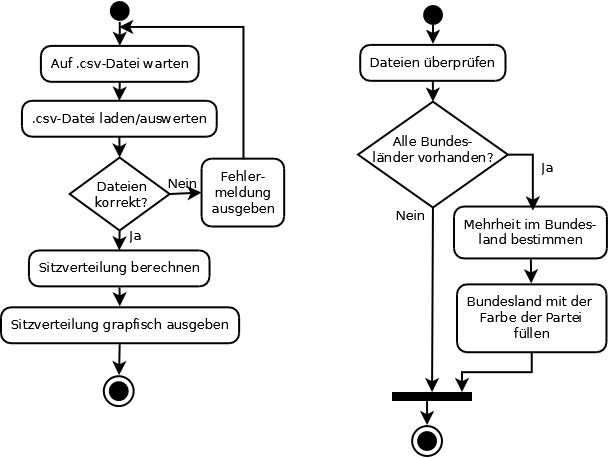
\includegraphics[scale=0.4]{Diagramm1} \\
Folgende Datenkonsistenzen müssen eingehalten werden:
\begin{itemize}
	\item noch nichts...
\end{itemize}
Folgende unzulässige Aktionen müssen korrekt behandelt werden:
\begin{itemize}
	\item Negative Stimmenanzahl
	\item Buchstaben als Stimmen
\end{itemize}
Testszenarien:
\begin{itemize}
	\item Falsche Daten importieren: \newline
	Starten des Programms $\rightarrow$ Im Hauptmenü auf Datei klicken $\rightarrow$ Datei importieren auswählen $\rightarrow$ Im Dateibrowser die falsche .csv-Datei auswählen $\rightarrow$ Mit dem Button Laden bestätigen $\rightarrow$ Eine Fehlermeldung taucht auf $\rightarrow$ Programm befindet sich wieder im Startzustand
	\item Manuell Daten modifizieren: \\
	Starten des Programms $\rightarrow$ Korrekte Daten laden $\rightarrow$ Die Sitzverteilung wird angezeigt $\rightarrow$ Den Wert zweier Parteien miteinander tauschen $\rightarrow$ Die Sitzverteilung erneut berechnen $\rightarrow$ Eine mögliche Veränderung der Sitzverteilung wird angezeigt
	
\end{itemize}
\section{Systemmodelle}
\subsection{Systemarchitektur}
Das Programm basiert auf der MVC- Architektur, wobei auf eine saubere Trennung der Einheiten Model, View und Controller geachtet wird. Dies sorgt nicht nur für einen flexiblen Programmentwurf, so dass spätere Änderungen bzw. Erweiterungen erleichtert werden, sondern garantiert auch die Trennung kritischer Komponenten, wie der Algorithmusimplementierung, von weniger sensiblen Komponenten, wie der GUI, und dient allgemein der Übersichtlichkeit.

\section{Benutzungsoberfläche}

\section{Spezielle Anforderungen an die Entwicklungsumgebung}
\begin{itemize}
	\item Allgemein
	\begin{itemize}
		\item Latex
		\item Versionskontrolle mit SVN
	\end{itemize}
	\item Entwicklung
	\begin{itemize}
		\item IDE: Eclipse
		\item GUI: Swing
	\end{itemize}
	\item Entwurf
	\begin{itemize}
		\item DIA für Diagramme
	\end{itemize}
	\item Validierung
	\begin{itemize}
		\item JUnit
	\end{itemize}
	\item Teamkommunikation
	\begin{itemize}
		\item Google-Groups Mailingliste
	\end{itemize}
\end{itemize}

\section{Zeit- und Ressourcenplanung}

\section{Ergänzungen}

\section{Glossar}



\end{document}
